\documentclass{article}
\usepackage[utf8]{inputenc}
\usepackage[version=4]{mhchem}
\usepackage{mathrsfs,relsize,makeidx,color,setspace,amsmath,amsfonts,amssymb}
\usepackage[table]{xcolor}
\usepackage{bm,ltablex,microtype}
\usepackage{placeins}
\usepackage{listings}
\usepackage[utf8]{inputenc}
\usepackage[top = 1in, bottom = 1in, right = 1in, left = 1in]{geometry}
\usepackage[pdftex]{graphicx}
\usepackage{blindtext}
\usepackage{MnSymbol,wasysym}
\usepackage{calrsfs}
\usepackage[mathscr]{euscript}
\usepackage{hyperref}
\usepackage{graphicx}
\usepackage{caption}
\usepackage{subcaption}
\usepackage{verbatim}

\newlength\tindent
\setlength{\tindent}{\parindent}
\setlength{\parindent}{0pt}
\renewcommand{\indent}{\hspace*{\tindent}}

\title{An Exercise in Planetary Destruction}
%Modeling the Solar System Through Velocity Verlet  \\ A Novel and Other Short Stories
\author{"Numpy" Nat Hawkins, Victor "Venv" Ramirez\\ "Matplotlib" Mike Roosa, Pranjal "Pandas" Tiwari}

\begin{document}

\maketitle
\begin{abstract}
In this project, we made a model of the orbits of the planets in our solar system and Pluto. The model was built using the Velocity Verlet algorithms, which uses numerical methods to create a system of four coupled differential equations. In this project we implemented methods of object oriented programming. This allowed us to reduce the code for the Verlet algorithm from around 500 lines of code to roughly 75 lines of code. This significant decrease demonstrated the power of object orientation in reducing our computation load as well as creating a more user-friendly program. The final product was a visualization  of our model for the solar system shown in Figure \ref{solar_system} below. Some additional investigation into the three body problem of Earth-Sun-Jupiter and how scaling of masses affects orbits was conducted and will be discussed in this report. We found some interesting cases where if the mass of Jupiter becomes too large, Earth will achieve escape velocity of the solar system. Similarly, we also were able to demonstrate the concept of escape velocity with an arbitrary "asteroid".
\end{abstract}

\begin{figure}[h!]
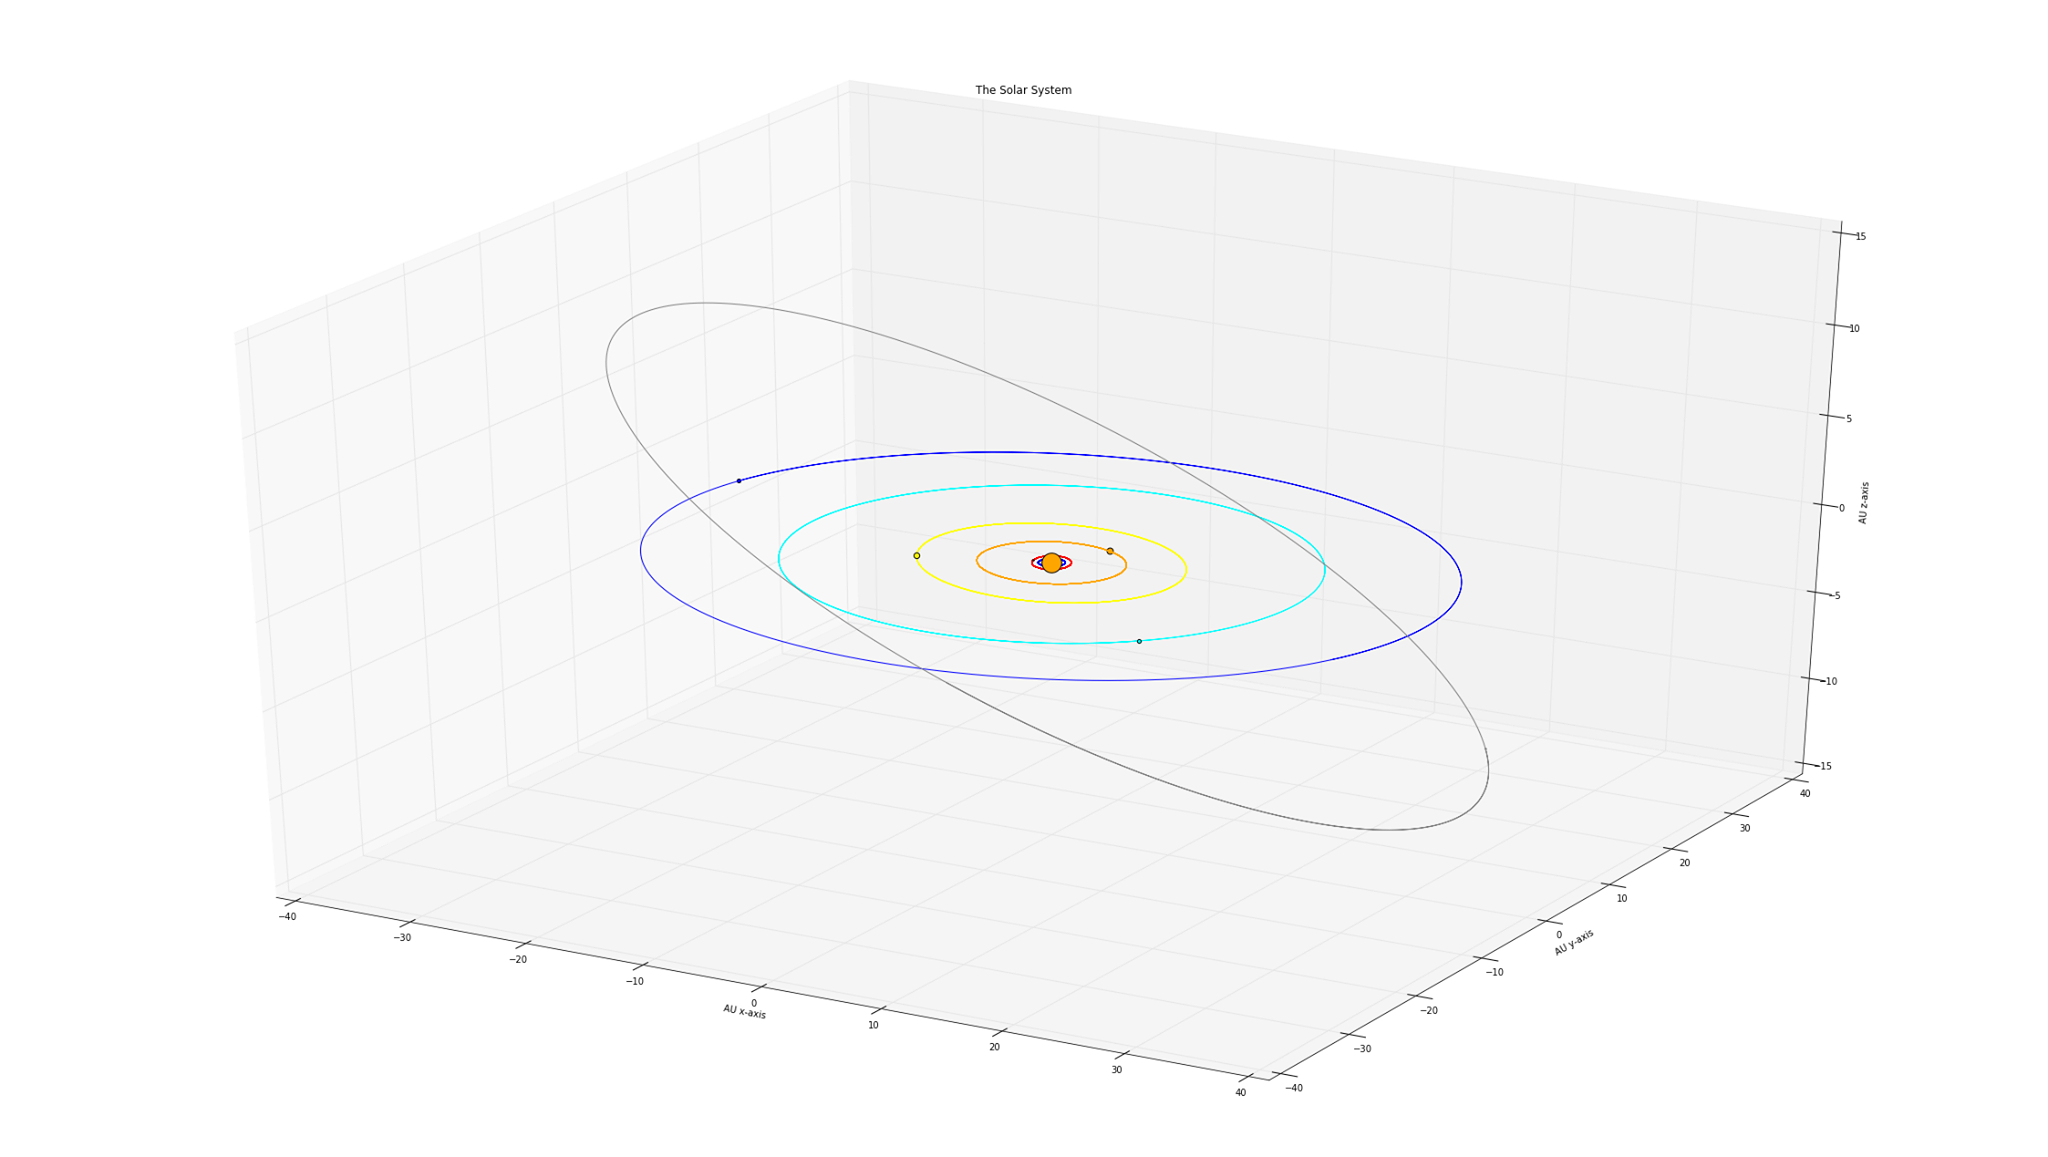
\includegraphics[width = \linewidth]{solar_system_pretty.png}
\caption{The final output of our solar system model with some fancy coloring and visual effects added. The plot shows the orbital paths of the planets of the solar system over the course of a full solar system orbital period (time required for all plates to complete a full revolution around the sun), which is $\approx$ 250 years. Visual created by our own Victor "Venv" Ramirez.}
\label{solar_system}
\end{figure}


\newpage

\section{Introduction}


\subsection{Motivation}
Throughout history, mankind has wondered about the motion of the sun, the planets, and whatever else is out there. Today, we can roughly simulate the Solar System with a computational power of a typical laptop. In this project, we modeled the Solar System by calculating the motion of the 9 historical planets and the Sun. We can calculate the motion by solving Newton's Laws of Gravitation using the popular Verlet Algorithm. Using this algorithm, and applying object oriented programming techniques, we created a fairly accurate model of the Solar System that is consistent with what we know about it. Although our program does not include additional objects like moons, large asteroid belts, etc., we feel that the accuracy is not hindered in any statistically significant way.

\subsection{Object Orientation}
Object orientation in this case is very useful, since we have to show the effects of all planets on one another for every time step. This will result in a multitude of equations that all have the same setup and only differ by the variables used. It made our code easier to read and likely more efficient.\\
A longer version of the code without object orientation \href{https://github.com/nathawkins/PHY480MSU/blob/master/project3/src/Python%20Files/hard_code_the_whole_shabang.py}{HERE}
. As you can see, this is a little ridiculous, upon closer inspection you may be able to see that the blocks of code are rather repetitive with small variations. Since this was all in a single function without any loops of any kind, it would be easy to think of a way to optimize this code. Doing so, would make the code much more readable to another user. Object orientation can be seen in affect in any of the final working codes. In regards to lessons we will carry forward, the use of object orientation will be a consideration whenever we deal with models of this level of complexity or models that have a similar nature of repetitive operation (as we will see, the equations for each planet look nearly identical with some rescaling of constants).

\section{Solution}

\subsection{Setup}
To begin this problem, we have to define the initial positions and velocities of the planets, which we got from NASA's JPL web-page \cite{JPL}. This data was then used to define where the planets are with respect to the sun. We used a class to actually define a "planet" with these initial positions and velocities. Then, we were simply able to update the information of the planet through referencing operations built into the class with the new position and velocity after every time step. \\
\\
Once the setup of the initial positions were set, we moved on to how the planets would react in the presence of the sun, which is the main contributor to the force acting on each planet. This was to ensure our code worked correctly and can be seen in the Two Planet case in the Results section (Figue \ref{earth_sun}). Understanding the importance of test cases, we performed a unit test where we included one more planet, Jupiter, into the program to ensure our equations worked properly prior to inlcuding all 9 planets in the code. This not only allowed us to ensure our numerical methods were correct, but it also gave us a new environment to perform additional unit tests in. These tests will be discussed in section 3.2 with the scalingof Jupiter's mass (Figure \ref{earth_wobble}) as well as the disucssion of escape velocity with making Jupiter's mass significantly larger (Figure \ref{earth go bye bye}). With these tests verifying our assumptions about how the gravitational force should alter orbits, we further expanded this to include all the planets and Pluto into our model.\\

\subsection{Method}
From a mathematical perspective, this project boils down to solving Newton's Second Law of Gravitation for our Solar System:
\begin{equation}
\frac{d^2x}{dt^2}=\frac{F_{G,x}}{M_{Planet}}
\end{equation}
The force in this case will need to account for the interaction between an object and every other object we are considering within the system. Through methods of scaling differential equations and the approximation to circular orbits, we were able to simplify down our constants:
\[
F_G= \frac{M_{\mathrm{Earth}}v^2}{r}=\frac{GM_{\odot}M_{\mathrm{Earth}}}{r^2},
\]
where $v$ is the velocity of Earth. The latter equation can be used to show that
\[
v^2r=GM_{\cdot}=4\pi^2\mathrm{AU}^3/\mathrm{yr}^2.
\]
This transformation allows us to rewrite our differential equation as 
\begin{equation}
\frac{dv_x}{dt} = \frac{-4 \pi^2}{r_E^3} x_E
\end{equation}
For a more thorough discussion of scaling differential equations, see Langtangen\cite{hpl text}. This is just a simple example equation for looking at the Earth-Sun interactions (assuming all masses scaled to multiples of the mass of the sun). There will be similar equations for the y acceleration and the z acceleration. This form is also repeated when it comes to looking at the interactions between the other planets and the sun. Here is an instance where we can write once and use many times.\\

To evaluate this ODE we need to first rewrite it as two coupled differential equation's. 
\begin{equation}
 \frac{dx}{dt}=v(x,t) \hspace{1cm}\mathrm{and}\hspace{1cm} \frac{dv}{dt}=F(x,t)/m=a(x,t)
\end{equation}
This allows us to easily evaluate the solution using a simple numerical method such as the velocity Verlet or RK4 method. Both will be discussed but we decided only to build simulations using the Verlet method for reasons which will be discussed later. 
\subsubsection{Many-Body gravitational force}
In order to accurately model the solar system we need to consider the interactions between the planets in addition to the force from the sun. Mathematically this entails adding interaction terms from each planet to the effective force equation. Interactions between Planet 1 and Planet 2 take the one dimensional form: 
\begin{equation}
 F_{x}^{1,2}=-\frac{GM_1M_2}{r_{1,2}^3}(x_1-x_2)
\end{equation}
When implemented, we rescaled the masses relative to the sun's mass which further simplifies our acceleration equations. 
\begin{equation}
F_{x}^{1,2} = \frac{-4 \pi^2 M_2/M_\cdot}{r^3_{1,2}} (x_1-x_2)
\end{equation}
As we include more bodies in our program, there will be additional terms added on to the acceleration of a planet for the interactions between whatever planet we are observing and the remainder of the planets in the solar system. 
\subsubsection{Verlet Solver}
Now that we have constructed an acceleration function for each planet, we can solve our equation. As stated earlier we relied on the Verlet method to produce our simulations. In parallel with our discussion in class\cite{morten github}, the Verlet method can be derived by considering th Taylor expansions of both the position and velocity functions: 
\begin{equation}
x_{i+1} = x_i+hx^{(1)}_i+\frac{h^2}{2}x^{(2)}_i+O(h^3)
\end{equation}
\begin{equation}
v_{i+1} = v_i+hv^{(1)}_i+\frac{h^2}{2}v^{(2)}_i+O(h^3)
\end{equation}
Now we can rearrange the velocity function to find an approximation of the jerk in terms of the acceleration:   
\begin{equation}
hv^{(2)}_i\approx v^{(1)}_{i+1}-v^{(1)}_i
\end{equation}
and substitute it into the velocity expansion. Recall, we have built an expression for the velocity derivative above. Together this lets us rewrite the position and velocity equations to the second order in terms of the acceleration equation. 
\begin{equation}
x_{i+1} = x_i+hv_i+\frac{h^2}{2}v^{(1)}_{i}+O(h^3)
\end{equation}
\begin{equation}
v_{i+1} = v_i+\frac{h}{2}\left( v^{(1)}_{i+1}+v^{(1)}_{i}\right)+O(h^3)
\end{equation}
These equations are very nice for our purposes because they can preserve energy conservation which will be discussed with more depth later.

\subsubsection{RK4}
RK4 is a very popular ODE solver we considered implementing for this project because of its simplicity and accuracy. That being said, its simplicity comes with some pretty serious draw-backs, specifically that it accumulates a global error. Because RK4 accumulates a global error it struggles to produce stable results, particularly in the context of problems where we want accuracy over many iterations. Although building an RK4 solver is relatively simple we decided not to implement it in a simulation for this reason favoring the stability of the Verlet solver to explore the physics of this system.

\section{Results}
\subsection{Earth-Sun Case}
Our first model was the two-body Earth-Sun system. In this system, the acceleration is only affected by the gravity of both bodies. In the figure below, the Earth's orbit follows a nearly perfect elliptical shape around the Sun, while the Sun remains relatively still. 

\begin{figure}[h!]
\centering
\includegraphics[width = 0.7\linewidth]{earth-sun.png}
\caption{The earth-sun system for a period of 5 years. Fortunately for us, this orbit is stable.}
\label{earth_sun}
\end{figure}
\subsection{Earth-Jupiter Case}
Figure \ref{earth_wobble} (Left) shows the Earth-Sun-Jupiter system. We wanted to first ensure that our algorithms would behave properly when we introduced additional bodies into the code. As discussed earlier, this was an opportunity for unit testing. Fortunately, this is also stable (at least for the immediate future). 

When looking at Jupiter with an increased mass, the motion of Earth will be perturbed by a nonzero amount. Having a Jupiter 10 times more massive as its original size would cause Earth's orbit to bend in a cyclical pattern depending on how close the two planets are to one another during the course of their orbits. This can be seen in Figure \ref{earth_wobble}. Notice how this alteration of the mass causes a change in the Earth's orbit.

With a Jupiter mass 1000 times its current mass, The Earth would be ejected out of the Solar System at a velocity above solar escape velocity. See Figure \ref{earth go bye bye}. This is discussed in the later section on escape velocity in greater detail.
\begin{comment}
old code for figures for both earth-jupiter cases
\begin{figure}
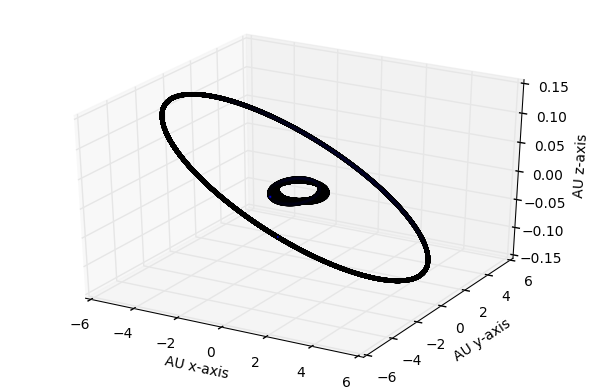
\includegraphics[width = 0.7\linewidth]{earth_moved.png}
\centering
\caption{The Earth-Jupiter-Sun system after 100 years. Here, the mass of Jupiter has been rescaled to 10 times its original mass. Notice how Earth's orbit has been altered as a result of the increased gravitational attraction.}
\label{earth_wobble}
\end{figure}

With a Jupiter mass 1000 times its current mass, The Earth would be ejected out of the Solar System at a velocity above solar escape velocity. See Figure \ref{earth go bye bye}. This is discussed in the later section on escape velocity in greater detail.

\begin{figure}[h!]
\centering
\includegraphics[width = 0.7\linewidth]{earth-sun-jupiter.png}
\caption{The Earth-Sun-Jupiter system for 50 years without mass scaling. Here, Earth's orbit remains constant.}
\label{earth_sun_jupiter}
\end{figure}
\end{comment}
\begin{figure*}[t!]

%\centering

\includegraphics[width=0.5\textwidth]{earth-sun-jupiter.png}
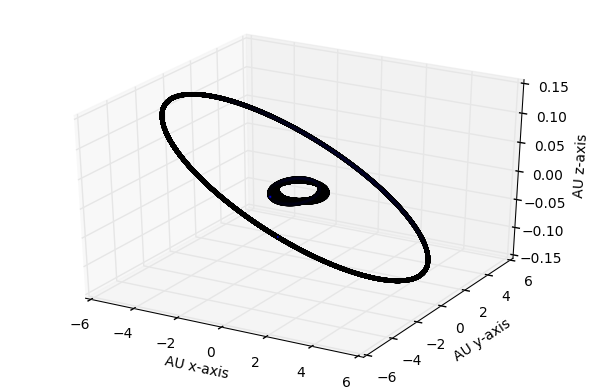
\includegraphics[width=0.5\textwidth]{earth_moved.png}
\caption{LEFT: The Earth-Sun-Jupiter system for 50 years without mass scaling. Here, Earth's orbit remains constant.
RIGHT: The Earth-Jupiter-Sun system after 100 years. Here, the mass of Jupiter has been rescaled to 10 times its original mass. Notice how Earth's orbit has been altered as a result of the increased gravitational attraction.}
\label{earth_wobble}
\end{figure*}

\subsection{All Planet Interaction Case}
The case where we included all planets into the program is very similar to the case with Earth and Jupiter, just with more planets. This is exemplified by Figure \ref{solar_system}, which has all the planets and includes the interactions they have with one another. We ran this program for 50 years and until that point, the program is observationally stable. Since most planets aren't moving at relativistic velocities, it would be safe to assume that the system would be stable for a period of time much longer than the tested 50 years. In Figure \ref{solar_system}, the period of time we iterated over was 250 years (approximately the orbital period of pluto), and we were able to observe stability, at least through our lifetimes.

\begin{figure}[h!]
\centering
\includegraphics[width = 0.7\linewidth]{first-few-planets.png}
\caption{A zoomed in image of the first few planets.}
\label{first_few_planets}
\end{figure}


\subsection{Conservation of Energy}
The Earth revolves around the Sun in an elliptical orbit, this would mean that the potential and kinetic energies relative to the sun would fluctuate in a cyclical pattern as shown in figure 5. shows that the kinetic and potential energies of the Earth do change over time. But something to note is that the sum of these two remains constant, which shows that energy is conserved for the Earth including all interactions from the other planets and Pluto. \\

\begin{figure}[h!]
\centering
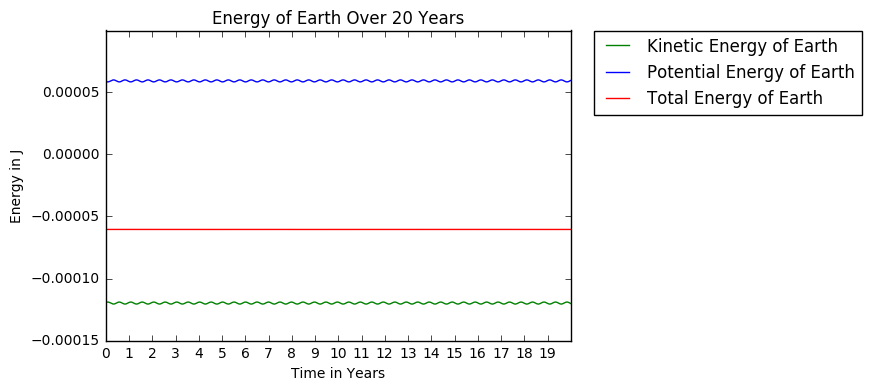
\includegraphics[width = 0.7\linewidth]{earth_energy.png}
\caption{Total Energy Diagram for Earth}
\label{earth energy}
\end{figure}

From what we can see, Mercury's orbit is much more elliptical than Earth's from the amplitudes in the oscillations of Mercury's Kinetic Energy as you can see from Figure 6. The total energy seems to be oscillatory as well, if we zoom in on it, as you can see from Figure 7, the total energy of Mercury does oscillate in a cyclic manner, but not in such a way that would correspond to a sine wave, which implies that there is an additional term to the energies that we have not included. Our speculation is that while both kinetic energy and potential energy are oscillatory, they do not "cancel" when we add them together, and some phase shift is causing us to observe this cyclical energy. We will have to make additional corrections to account for this, but as you can see from the y-axis of this graph, the change in total energy is not very large and doesn't seem to change over a period of time, so unless we let the program run for a very long time, on the order of one million years, the solar system as a whole will stay stable.

\begin{figure}
  \centering
  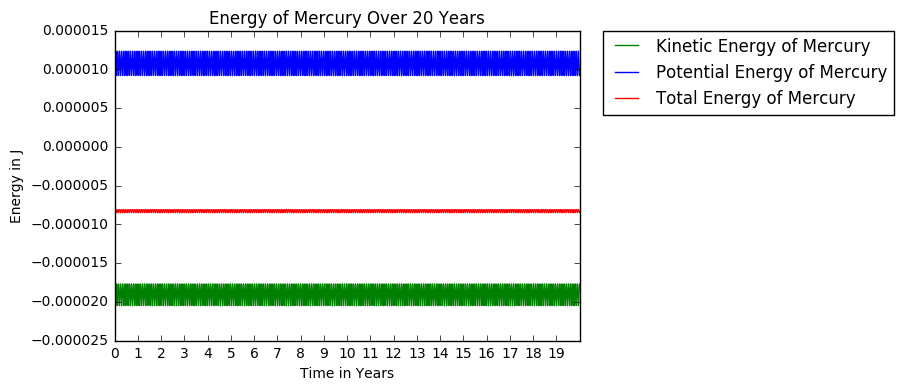
\includegraphics[width=0.9\linewidth]{mercury_energy.png}
  \caption{Energy Diagram for Mercury. The key indicates the type of energy being plotted. Notice how the red line, indicating total energy, does not appear to be a line at constant value.}
  \label{mercury energy}
\end{figure}
\begin{figure}
  \centering
  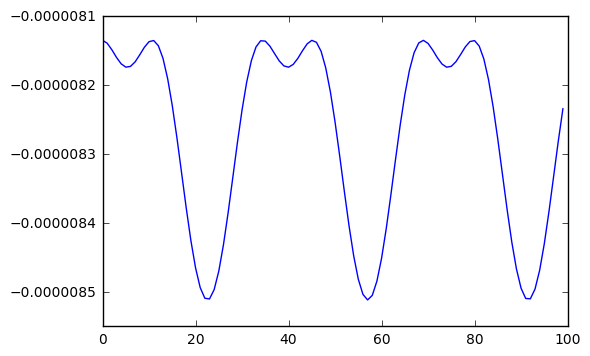
\includegraphics[width=0.7\linewidth]{zoom_in_mercury.png}
  \caption{Total Energy of Mercury. This is a more focused or zoomed in view of the "red line" (total energy) from Figure \ref{mercury energy}. The y-axis denotes the energy of the planet, and the x-axis is again time. We see that the total energy is now also periodic, and not a constant value as we would expect. Though it is important to note that the energy only fluctuates by a small margin. Some additional correction to our code is needed to improve the accuracy of this model and give us the expected constant total energy for Mercury.}
  \label{zoom in}
\end{figure}


\subsection{Escape Velocity}

We began by programming in an object (we will refer to it as an asteroid for the purpose of this discussion). The asteroid begins at approximately 1 AU from the Sun. We chose to put it at 1 AU in the x-direction, and 0 AU in both the y and z directions. This was just an arbitrary choice for the sake of the program, but we could have chosen to make any coordinate choice. According to \cite{escape velocity}, we calculate escape velocity through the following equation:
\begin{equation}
v_{escape} = \sqrt{\frac{2 G M}{R}}
\end{equation}
For the sake of finding the escape velocity, we used a similar approach and scaled $GM_\odot \approx 4 \pi^2$. This simplified our calculation of the escape velocity to a numeric result of approximately $v=\sqrt{8 \pi^2}$ AU/year. We chose to let this object travel in the x-direction with this velocity to see if it will escape with this numerical result.\\

Figure \ref{escape} shows the asteroid escaping the solar system. The scales of the axes changed dramatically. We can see the asteroid flies past the outer orbit of the solar system. In regards to our numerical result calculated based on what we know about escape velocity, this demonstrates the concept effectively. We can see an object starting at approximately 1 AU from the sun can escape the inner solar system for sufficient velocity. Notice the sheer distance that the object covers over the 250 year period that the program compiled over. This was also demonstrated when we scaled the mass of Jupiter in the Earth-Jupiter to system to be 1000 times its original mass. Figure \ref{earth go bye bye} shows that after 100 years with Jupiter's mass scaled closer to being that of the mass of Sun, then we can actually accelerate Earth to escape velocity. \\

This demonstrates the concept of escape velocity in a very interesting way. Looking at planetary motion in upper limits where planets literally fly off into deep space is analogous to objects leaving Earth. With this analogy in mind, and knowing we can show it in our simulation, we can discuss some commercial aspects of launching objects into space in the future. See "Future Additions" section for discussion on this.

\begin{figure}[h!]
\centering
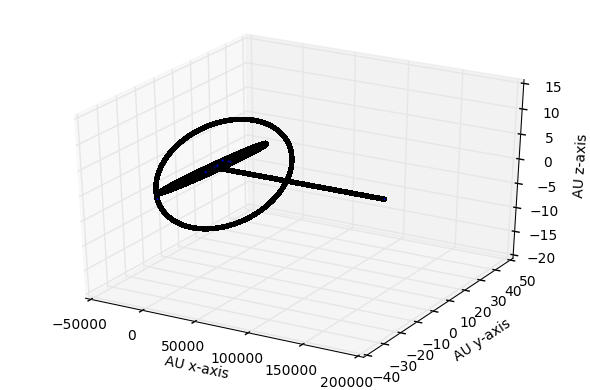
\includegraphics[width = 0.7\linewidth]{escape.png}
\caption{Object achieving escape velocity for the Sun. Beginning 1 AU from the Sun. Note the scale on the x-axis.}
\label{escape}
\end{figure}


\begin{figure}[h!]
\centering
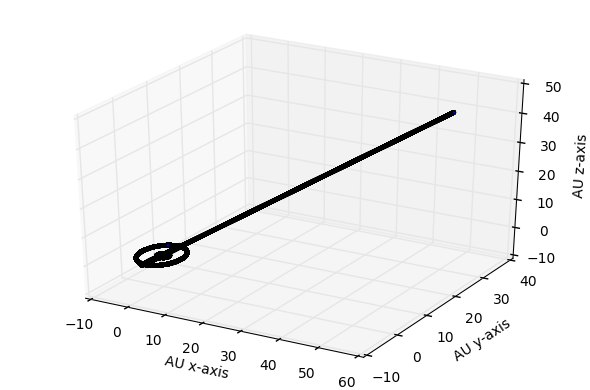
\includegraphics[width = 0.7\linewidth]{throw_da_earth.png}
\caption{Earth being accelerated to escape velocity after we rescale the mass of Jupiter 1000 times its original mass. Simulation time: 100 years.}
\label{earth go bye bye}
\end{figure}

\section{Future Additions}
This model of the solar system is decent, but there are some more inclusions to the program that could be made to give a more accurate representation of the solar system.\\

For starters, we could include more bodies into the code. The code is set up so that adding a body is simply just inputting the data from NASA and JPL, and run it through our "makeplanet" class. Then, we append it to the array of other planets and have the Verlet solver include that in the algorithmic iterations. The inclusion is simple, but as we saw with the Earth-Jupiter-Sun system, including different masses can have an effect on the orbit of a planet as Jupiter's mass in certain circumstances was able to alter Earth's orbit by a non-zero amount. The inclusions could range from very simple to very computationally dense. We could include Earth's moons as well as the numerous moons of Jupiter and Saturn into our code. More complex additions could include asteroid belts, the rings of Saturn, and even additional solar systems in the neighboring Milky Way galaxy. The possibilities are endless when it comes to what more we could add to this code. As we make it more aligned with the "real world" solar system, we would still hope to see the same level of stability for at least so long as we're alive\\

We could continue our analysis by including relativistic effect into our code. We know the Mercury processes due to some relativistic corrections, and including more bodies into this code may include the addition of high velocity bodies or systems, also under the influence of relativistic effects. Correcting for relativistic effects provide a small but non-trivial adjustment for the planets, but may be more important for including celestial bodies that are moving faster, such as asteroids.  \\

Some practical things to introduce to the code would be human exploratory efforts. Since we have a working model of the solar system, we could use this to some rough extent to plot the trajectory of an object being launched into deep space, or being put into orbit around a planet, or surveying a nearby galaxy. This model allows us to map motion outside of the realm of human interactions, and from a commercial standpoint, that is a valuable tool when considering launching multi-million dollar satellites or probes into space. This is a computational tool that, given some initial parameters or small adaptations, can be included in our model very easily.\\

Integration to more complex software would be the next step from a computational standpoint. This was all coded on personal laptop computers with commercially available processor power and memory. Integrating this into some more elaborate software with higher processing power and CPU space could  yield faster calculations for larger scale systems. If there were some way to integrate this into a visual output software, we could make a model that updates in real time and visually updates. Our current model outputs one 3 dimensional plot at the end of whatever time frame we tell the program to run over. Being able to actually see the motion unfolding adds another dimension to the interaction between programmer and program, and could be an interesting software development project. \\

\section{Conclusion}
The Verlet Algorithm provides a fairly accurate method to simulate the motion of the historical planets. The orbits are stable within the timescale of about 10$^2$ years, but simulations for longer periods of time would, perhaps, would be able to answer the question of long term-stability of the solar system. The energies for most of the bodies remain conserved, however Mercury's energy showed some fluctuations due to some additional effects that we did not take into account when building our model. This project gave insight into using object oriented programming techniques to significantly streamline the process of tracking the motion of the planets and the use of this programming technique as a whole. Although our model only consists of the 9 historical planets, it provides the foundation that allows us to expand this model by adding more celestial bodies, such as the moons, asteroids, and on a much larger scale other solar systems.


\begin{thebibliography}{9}
	\bibitem{morten github} Discussions and Lecture Slides on Ordinary Differential Equations. Morten Hjorth-Jensen. \url{https://compphysics.github.io/ComputationalPhysicsMSU/doc/pub/ode/html/ode-reveal.html}. GitHub. 
    
    \bibitem{hpl text} Hans Petter Langtangen. \textit{Scaling of Differential Equations}. Source: \url{http://hplgit.github.io/scaling-book/doc/pub/book/html/._scaling-book000.html}. GitHub. 2016.
    
    \bibitem{JPL} Solar System Dynamics. HORIZONS Web-Interface. \url{https://ssd.jpl.nasa.gov/horizons.cgi#top}. Jet Propulsion Labratory. NASA.
    
    \bibitem{wikipedia} Wikipedia. \textit{Newton's Law of Universal Gravitation}. \url{https://ssd.jpl.nasa.gov/horizons.cgi#top}. 
    
    	\bibitem{escape velocity} Discussion on Escape Velocity. HyperPhysics. \url{http://hyperphysics.phy-astr.gsu.edu/hbase/vesc.html}. 
    
    \bibitem{conservation of energy} Discussion of Conservation of Energy. \url{https://www.khanacademy.org/science/physics/work-and-energy/work-and-energy-tutorial/a/what-is-conservation-of-energy}. Khan Academy.
\end{thebibliography}


\end{document}